\documentclass[12pt]{article}
\usepackage{cite}
\usepackage{graphicx}
\usepackage{geometry}
\usepackage{float}
\usepackage{multicol}

\geometry{left=2.0cm,right=2.0cm,top=2.5cm,bottom=2.5cm}

\title{
    \textbf{\Huge ECE385} \\
    \huge Fall 2020 \\
    \huge Experiment 3 \\[120pt]
    \textbf{\Huge A Logic Processor} \\[120pt]
    }

\author{
    \large Name: Zhou Qinren \\ 
            \quad\qquad Zhang Yichi \\
    \large Lab Section: LA3 \\
    \large TA's Name: Yu Yuqi
    }

\date{Oct. $12^{nd}$ 2020}

\begin{document}
\setlength{\parindent}{0pt}
\maketitle
\newpage

\section{Introduction}
\subsection{functions and operations}
Our circuit is a bit-serial logic operation processor, with two 4-bit registers as the input. The processor can perform eight different functions, including bitwise AND, OR, XOR, NAND, NOR, XNOR, 1111 and 0000, on the 4-bit inputs. The result can be stored into whichever register we want, depending on our instruction.
\subsection{pre­lab questions}
Question: Describe the simplest (two-input one-output) circuit that can optionally invert a signal (i.e., one input determines if the output is equal to the other input or equal to the other input inverted). Sketch your circuit. \\

Answer: Assume the input signal is S, and the control signal is C. The output signal Q is equal to S if C is false, and the inverted S if C is true. \\
The logic is as follows: \\
$Q = S\overline{C} + \overline{S}C$ \\
In fact, this logic is the same as S XOR C. \\
Diagram: \\
\begin{figure}[H]
    \centering
    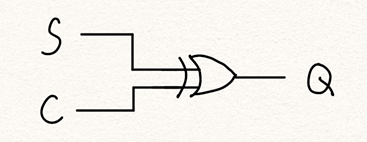
\includegraphics{prelab.png}
\end{figure}
Question: Explain how a modular design such as that presented above improves testability and cuts down development time. \\

Answer: A module design frees us from the burden of understanding the detailed circuit design. With a module design, we shall only focus on the input and output signals of the module, and treat the module as a black box. If everything inside the black box behaves exactly as what we expect, then we do not have to memorize what gates and how they are placed inside the module. Therefore, development time can be reduced by a large amount. Moreover, if we find a module behaves well when debugging, then we know the bug is at somewhere else.

\section{Operation of the Logic Processor}
\subsection{load data}
Load data into register A:  Set the input data by flipping switches D3-D0. Then turn on Load A, the data will flow into the register from D3-D0. \\
Load data into register B:  Set the input data by flipping switches D3-D0. Then turn on Load B, the data will flow into the register from D3-D0.

\subsection{initiate a computation and routing operation}
Set the function mode by flipping switches F2 F1 F0 and set the routing mode by flipping switches R1 R0. Then turn on the switch Execute, the computation begins. 

\section{Written Description, Block Diagram and State Machine Diagram of Logic Processor}
\subsection{written description}
The register unit contains two 4-bit registers to store the value to be calculated, one for the value A named RegA, another for the value B named RegB. They send the data to computation unit to do the calculation one bit at a time. \\

The computation unit can implement 8 kinds of desired calculation: and, or, xor, output 1, nand, nor, xnor, output 0. It calculates and sends the result (1 bit) together with the original two bits from A and B to the routing unit. \\

The routing unit sends the result back to the register unit. There are four patterns to be chosen. It is available to store the result to A or to B or keep the A and B or switch the A and B. \\

The control unit decides the working state of the logic processor. When it is in its reset state, it resets the counter and do nothing. When it is in its shift/hold state, it does the calculation, shifts to update or holds the data in the register unit according to the routing unit.

\subsection{high-level block diagram}
\begin{figure}[H]
    \centering
    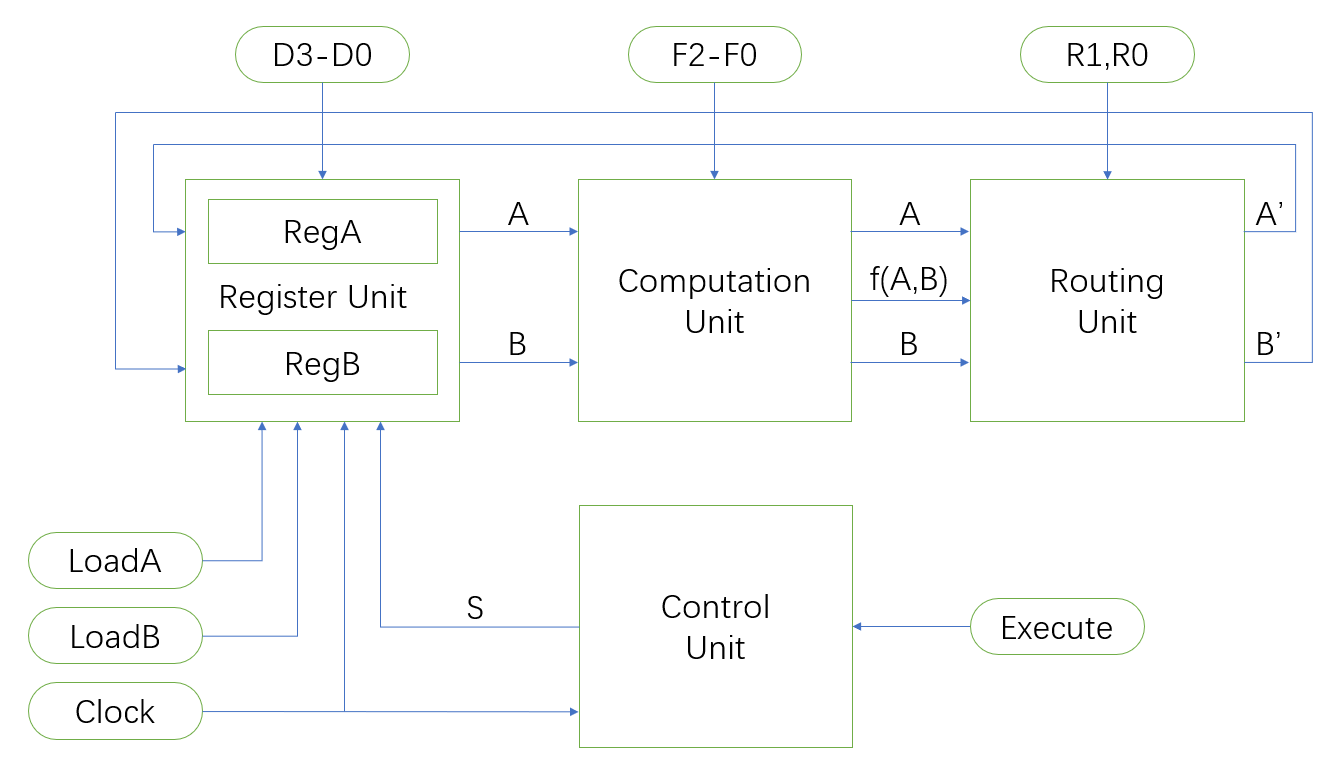
\includegraphics[width=18cm]{high_level_diagram.png}
    \caption{high level block diagram}
\end{figure}
\begin{figure}[H]
    \centering
    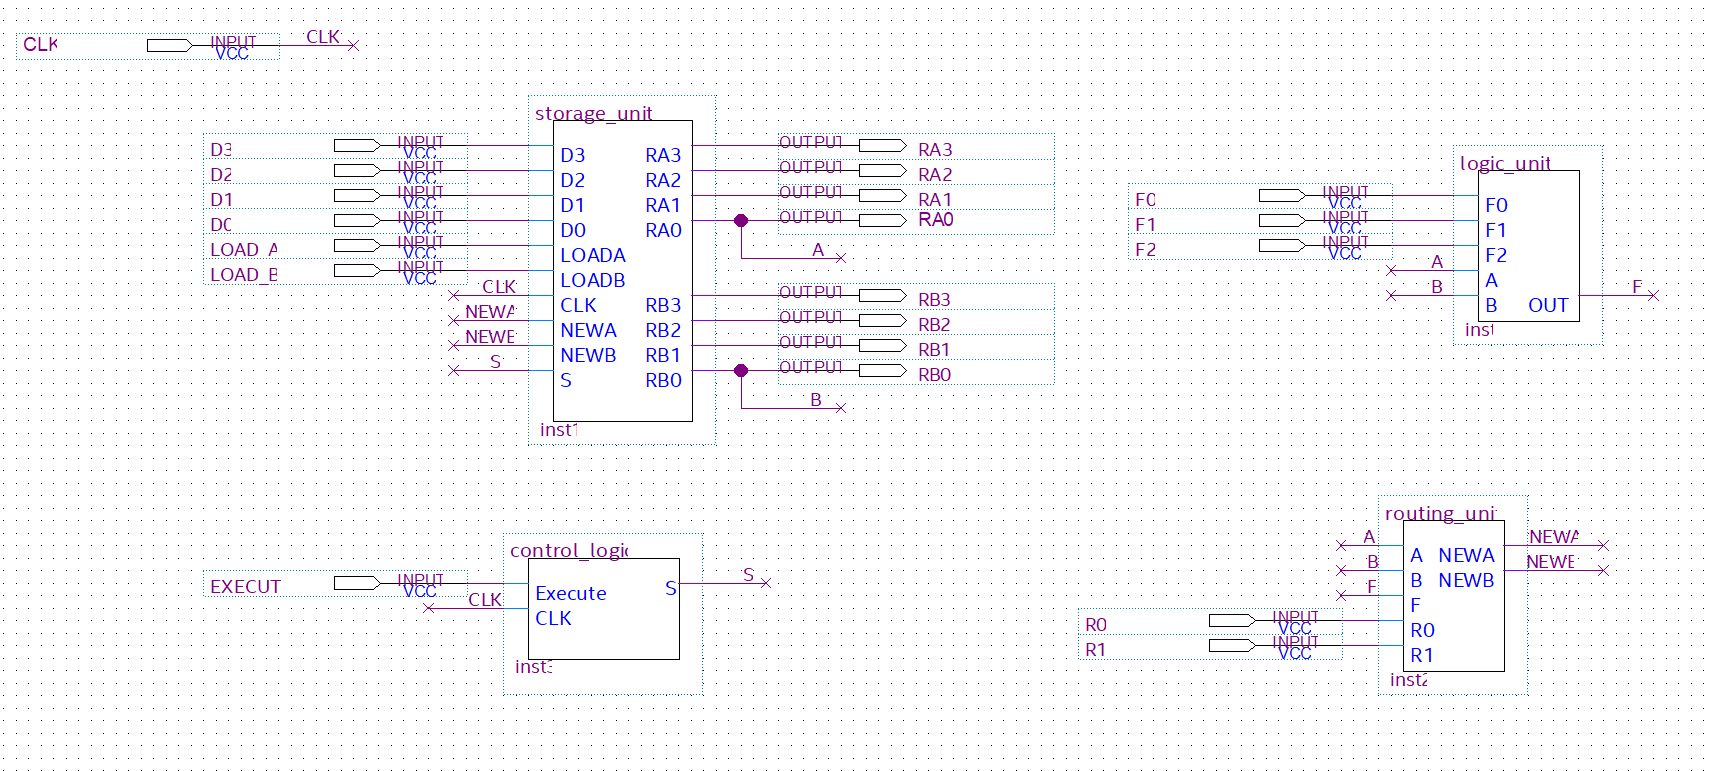
\includegraphics[width=18cm]{top_level_circuit.png}
    \caption{top level circuit diagram}
\end{figure}
\subsection{state machine diagram}
\begin{figure}[H]
    \centering
    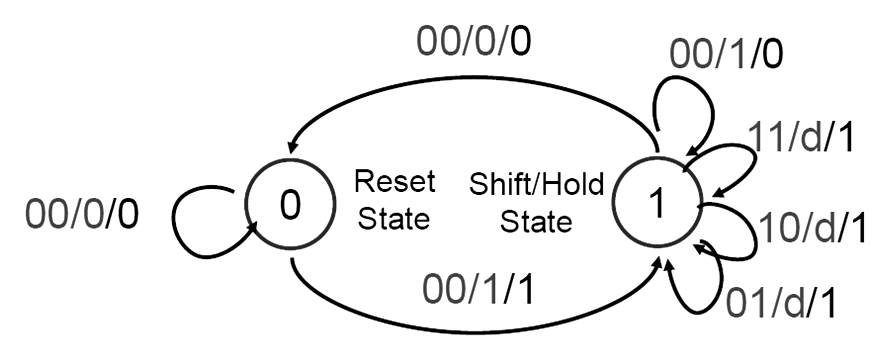
\includegraphics[width=18cm]{state_diagram.png}
    \caption{state machine diagram \cite{GG}}
\end{figure}
Arc label: \\
count(C1C0)/execute(E)/shift(S) \\

We use the Mealy machine with two states, 2 inputs, 1 bit output. We use 1 bit Q to represent two states. When $Q=0$, the processor is in the reset state. When $Q=1$, the processor is in the shift/hold state. Inputs are a 2 bits counter (C1C0) and an execute signal (E) which triggers the whole process of passing data, calculation, storage and so forth. The counter is a regular 2-bit counter from 00 to 11. The output is shift signal (S) which allows the processor to load values A and B from the outside.


\section{Design Steps Taken and Detailed Circuit Schematic Diagram}
\subsection{written procedure of the design steps taken}
\begin{table}[H]
    \centering
    \begin{tabular}{|cccc|cccc|}
    \hline
    E & Q & C1 & C0 & S & $Q^+$ & $C1^+$ & $C0^+$ \\ \hline
    0 & 0 & 0  & 0  & 0 & 0     & 0      & 0      \\
    0 & 0 & 0  & 1  & d & d     & d      & d      \\
    0 & 0 & 1  & 0  & d & d     & d      & d      \\
    0 & 0 & 1  & 1  & d & d     & d      & d      \\ \hline
    0 & 1 & 0  & 0  & 0 & 0     & 0      & 0      \\
    0 & 1 & 0  & 1  & 1 & 1     & 1      & 0      \\
    0 & 1 & 1  & 0  & 1 & 1     & 1      & 1      \\
    0 & 1 & 1  & 1  & 1 & 1     & 0      & 0      \\ \hline
    1 & 0 & 0  & 0  & 1 & 1     & 0      & 1      \\
    1 & 0 & 0  & 1  & d & d     & d      & d      \\
    1 & 0 & 1  & 0  & d & d     & d      & d      \\
    1 & 0 & 1  & 1  & d & d     & d      & d      \\ \hline
    1 & 1 & 0  & 0  & 0 & 1     & 0      & 0      \\
    1 & 1 & 0  & 1  & 1 & 1     & 1      & 0      \\
    1 & 1 & 1  & 0  & 1 & 1     & 1      & 1      \\
    1 & 1 & 1  & 1  & 1 & 1     & 0      & 0      \\ \hline
    \end{tabular}
    \caption{truth table}
\end{table}
\begin{figure}[H]
    \centering
    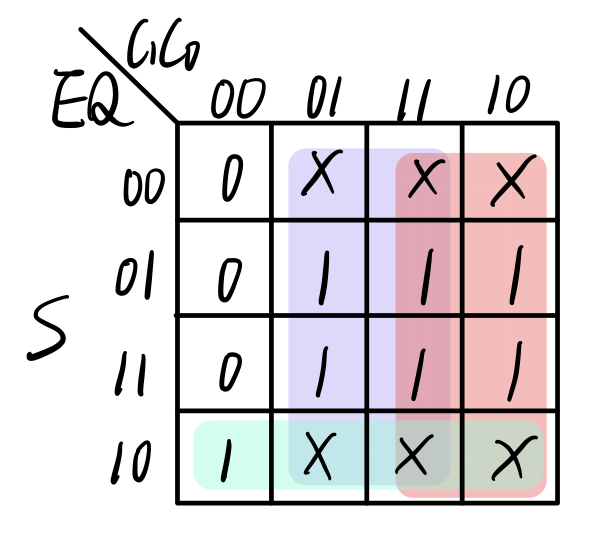
\includegraphics[width=8cm]{S.png}
    \caption{K-map for S, $S=C1+C0+E\overline{Q}$}
\end{figure}
\begin{figure}[H]
    \centering
    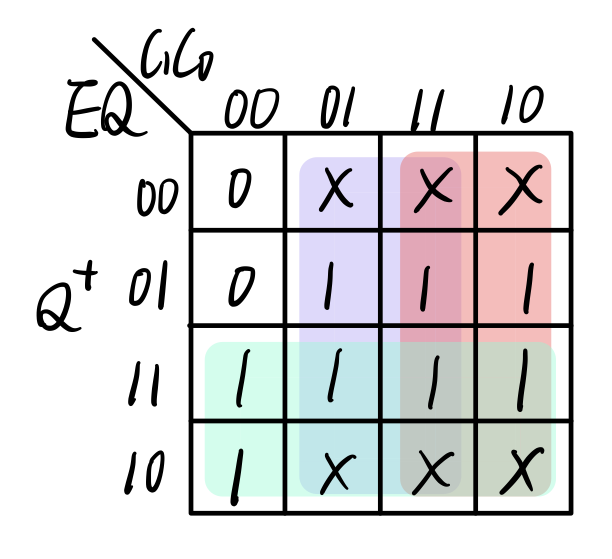
\includegraphics[width=8cm]{Q+.png}
    \caption{K-map for $Q^+$, $Q^+=C1+C0+E$}
\end{figure}
\begin{figure}[H]
    \centering
    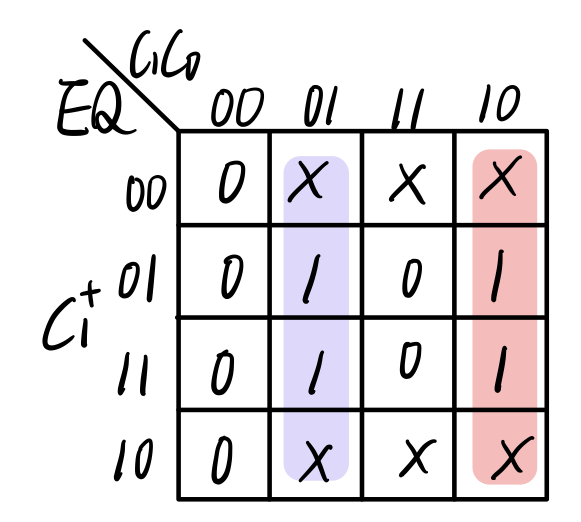
\includegraphics[width=8cm]{C1+.png}
    \caption{K-map for $C1^+$, $C1^+=\overline{C1}C0+C1\overline{C0}=C1 \oplus C0$}
\end{figure}
\begin{figure}[H]
    \centering
    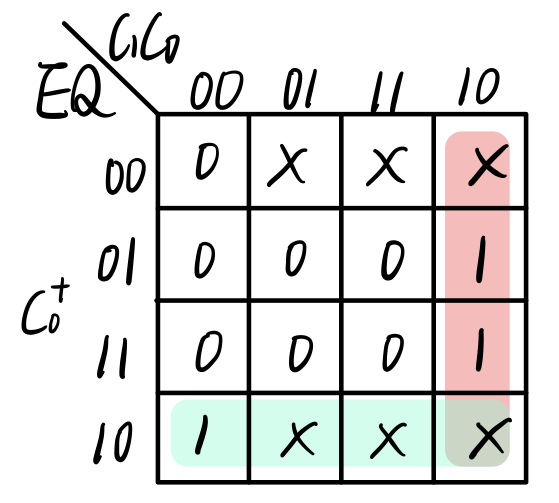
\includegraphics[width=8cm]{C0+.png}
    \caption{K-map for $C0^+$, $C0^+=\overline{C1}C0+E\overline{Q}=\overline{\overline{\overline{C1}C0}\ \overline{E\overline{Q}}}$}
\end{figure}
We use a Mealy machine to construct our core design rather than a Moore machine to reduce the number of states. It takes the risk of unintentional pulse but largely decrese the complexity of the logic and circuit which we would consider as worthy. Also, we move the LoadA and LoadB to the register unit to make the design clearer. In this design, only the signal execute (E) can turn the state from reset to shift/hold which simplifies the whole process. Right after it goes to the shift/hold state, it will automatically run 1 hold and 3 shift process to do the calculation of the 4-bit values A and B not caring the excecute signal.


\subsection{detailed Circuit Schematic}
\begin{figure}[H]
    \centering
    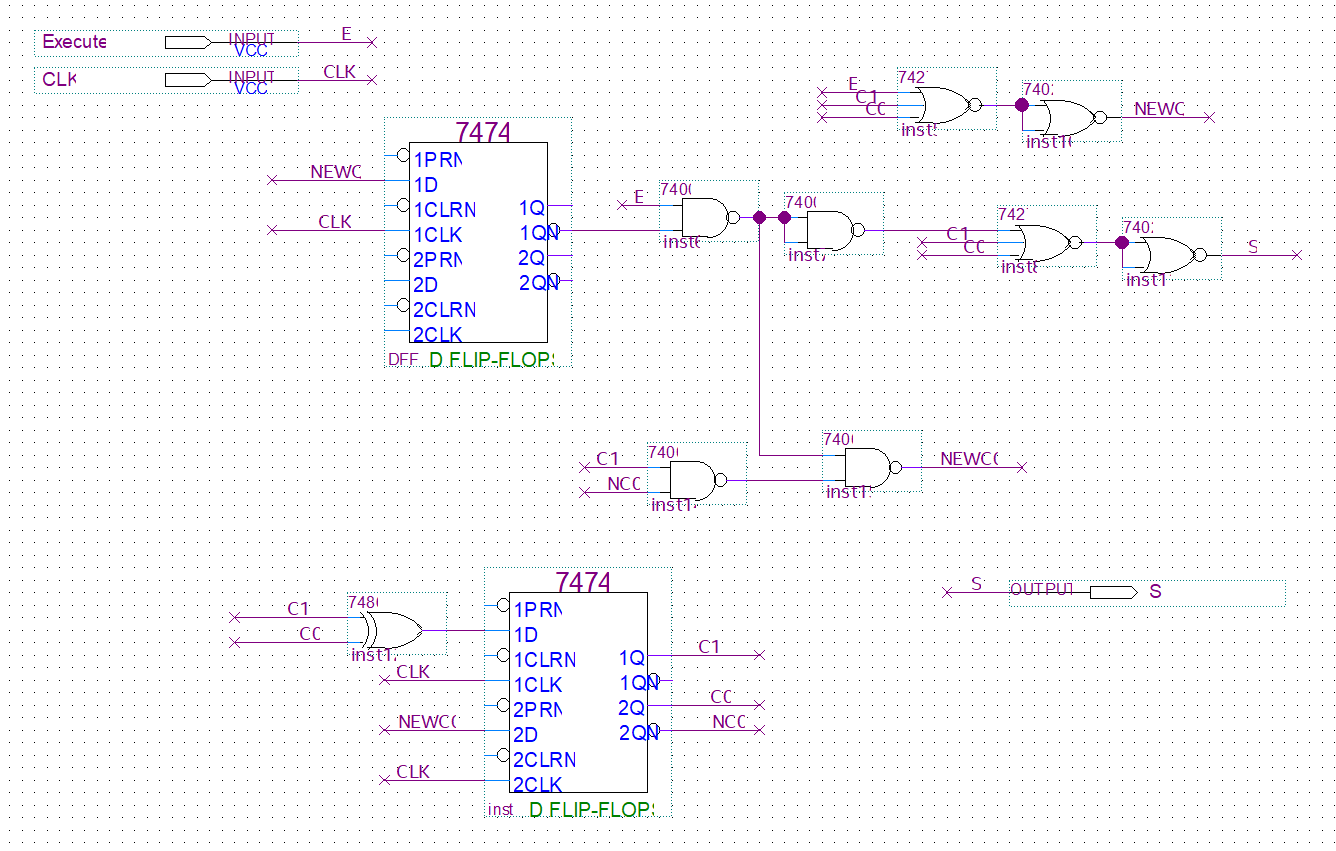
\includegraphics[width=18cm]{control_unit.png}
    \caption{control unit}
\end{figure}
\begin{figure}[H]
    \centering
    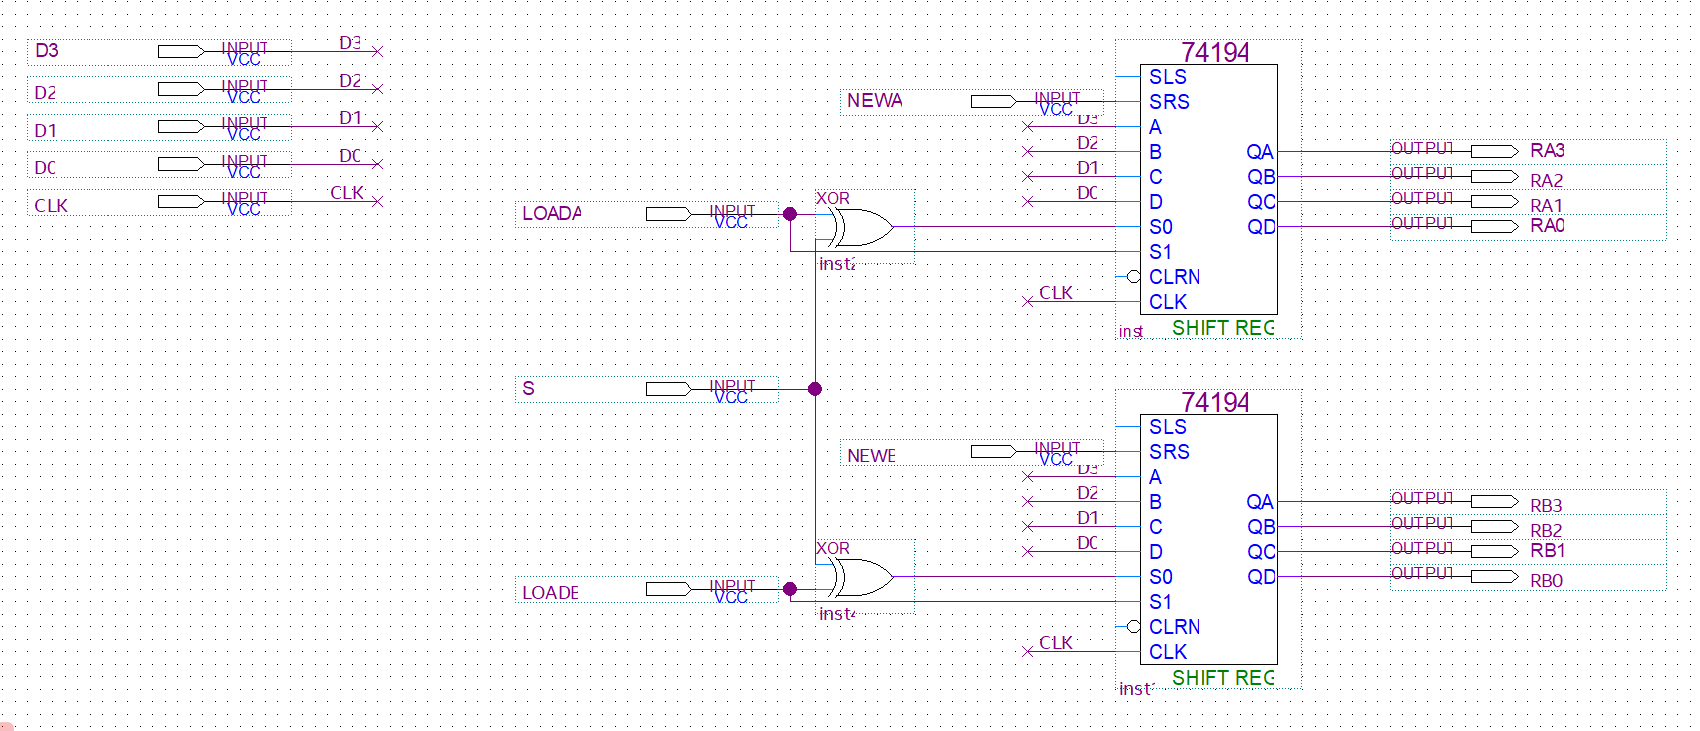
\includegraphics[width=18cm]{register_unit.png}
    \caption{register unit}
\end{figure}
\begin{figure}[H]
    \centering
    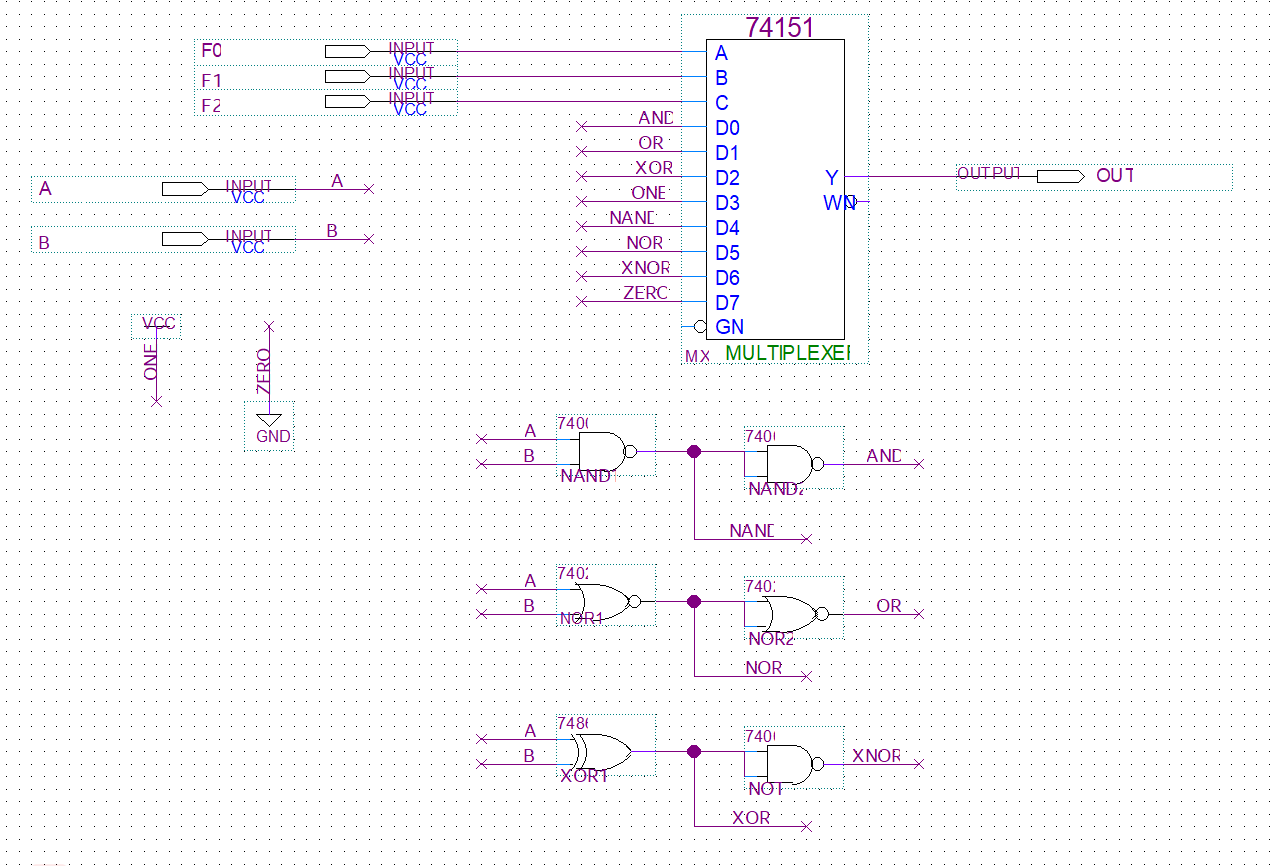
\includegraphics[width=16cm]{computation_unit.png}
    \caption{computation unit}
\end{figure}
\begin{figure}[H]
    \centering
    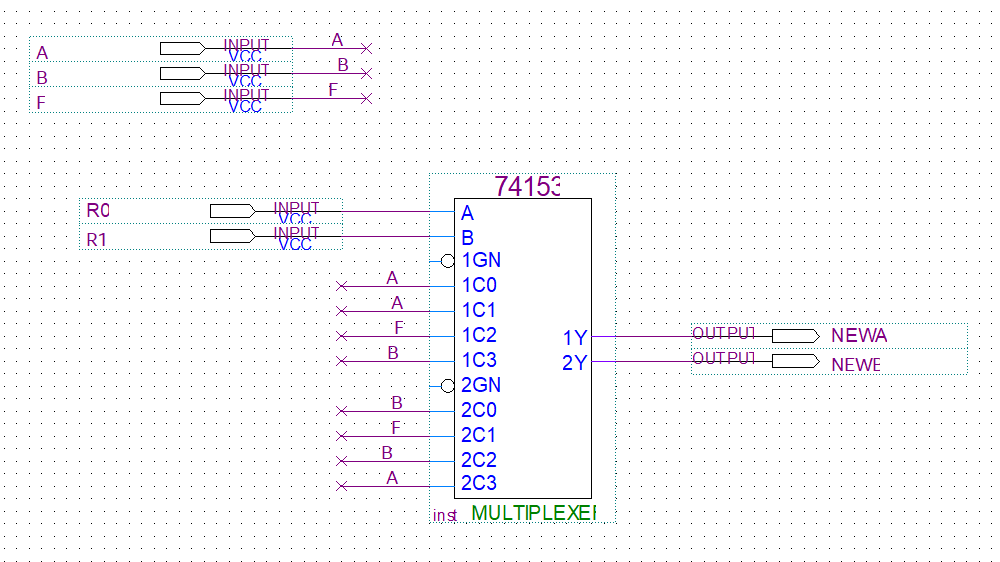
\includegraphics[width=15cm]{routing_unit.png}
    \caption{routing unit}
\end{figure}

\section{Description of All Bugs Encountered, and Corrective Measures Taken}
Since we make use of the idea of module design, our construction and debugging process hardly encounters difficulty. The only bugs are due to the wrong connections of wires when connecting the different modules, and it did not take too much work to find out the bugs, thanks to the modular approach.

\section{Conclusion}
\subsection{summarization}
In this lab, we learn to use Quartus to design and construct a 4-bit serial processor. The modular approach greatly shortens our development time and reduces the potential bugs. We also designed a Mealy machine to control the register unit. The Mealy machine makes the output dependent on both the input and the current state, minimizing the number of states. 

\subsection{post-lab questions}
Question: Outline how the modular approach proposed in the pre-lab help you isolate design and wiring faults, be specific and give examples from your actual lab experience. \\

Answer: The modular approach greatly helps the development process. For a concrete example, we generally divide the circuit into four parts: control unit, routing unit, register unit and computation unit. When a bug shows up, we can test each unit first, and decide whether each unit is functioning appropriately. If so, then we know the bug is at somewhere else, and turn to another unit for test. \\

Question: Discuss the design process of your state machine, what are the tradeoffs of a Mealy machine vs a Moore machine? \\

Answer: The design process of the state machine mainly consists of three parts: firstly, recognizing the related input, secondly, specifying the states representation, and finally, calculate the transition logic and output logic by K-map. \\
We noticed the only relevant input is the Execute signal, which instructs our processor to perform a function. When specifying the states, we found that we need a counter so as to count the number of elapsed clock cycles. But in order to reduce the number of states, we decided to use a Mealy machine, and add two new input C1 and C0, which serves as the counter. \\ 
The advantage of a Mealy machine over a Moore machine is that Mealy machine usually has fewer states, since the output not only depends on the current states but also the inputs. As the input carries information, the state machine can be constructed with fewer states if we make use of that information. The disadvantage of the Mealy machine is that it sometimes causes a clock issue if we make a bad design. The state is synchronous with the clock, but the input is not, therefore, some logic consisting of the input and state may cause an unintentional pulse.


\section{Waveform Generated by the Standard Testing Input}
\begin{figure}[H]
    \centering
    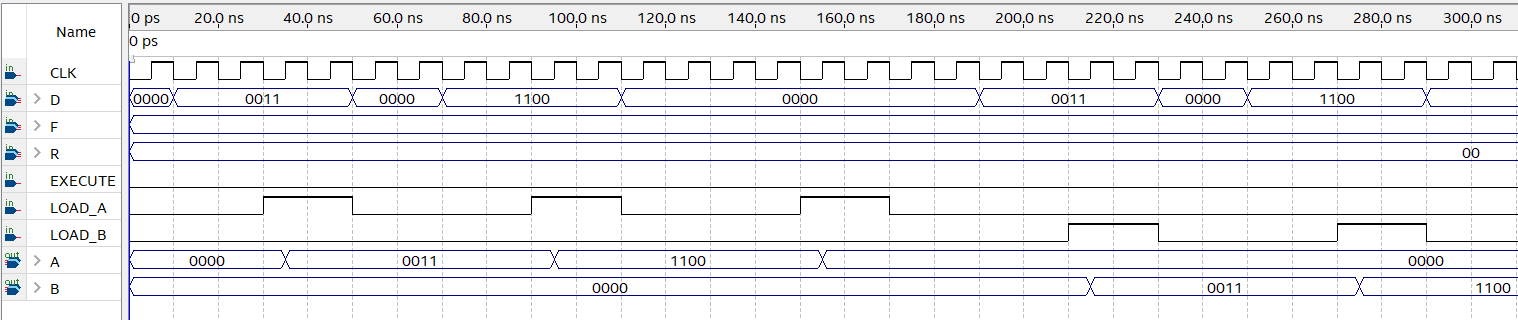
\includegraphics[width=18cm]{0-300.png}
    \caption{0-300ns}
\end{figure}
\begin{figure}[H]
    \centering
    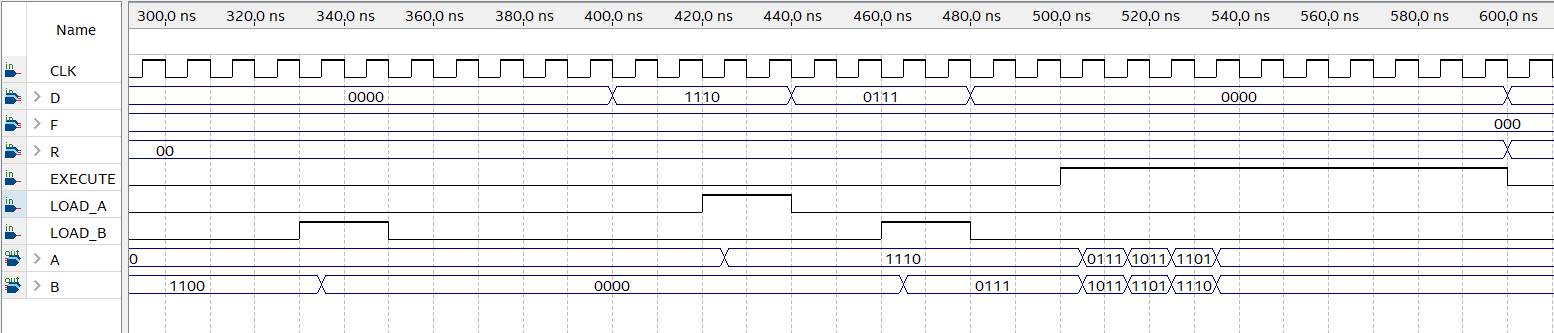
\includegraphics[width=18cm]{300-600.png}
    \caption{300-600ns}
\end{figure}
\begin{figure}[H]
    \centering
    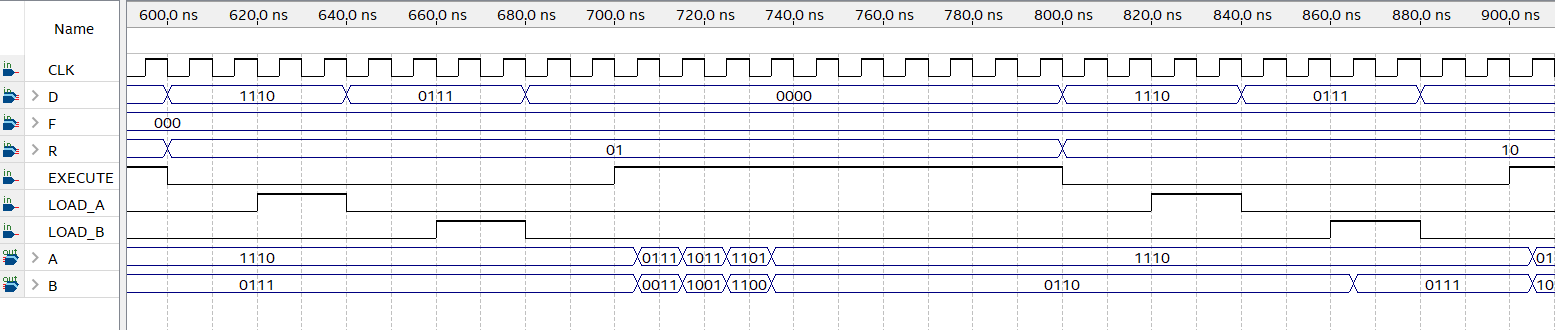
\includegraphics[width=18cm]{600-900.png}
    \caption{600-900ns}
\end{figure}
\begin{figure}[H]
    \centering
    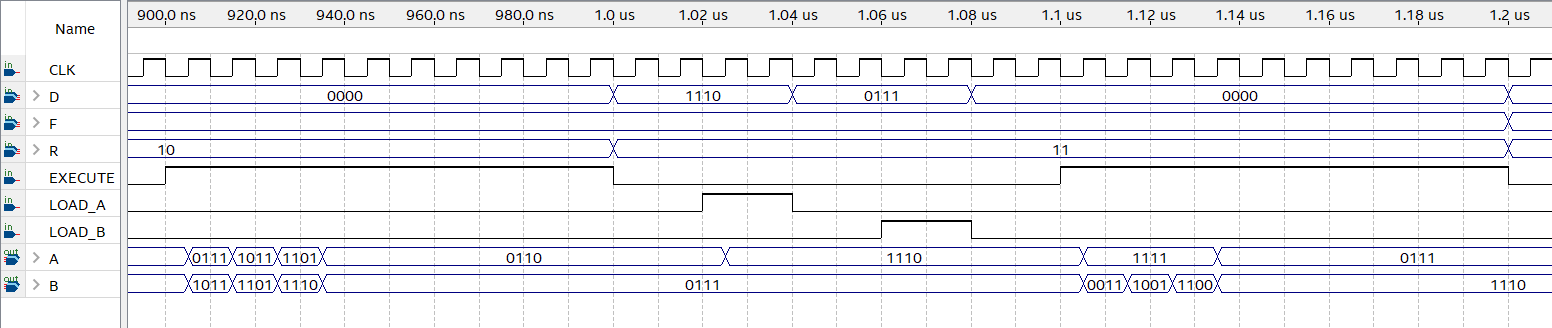
\includegraphics[width=18cm]{900-1200.png}
    \caption{900-1200ns}
\end{figure}
\begin{figure}[H]
    \centering
    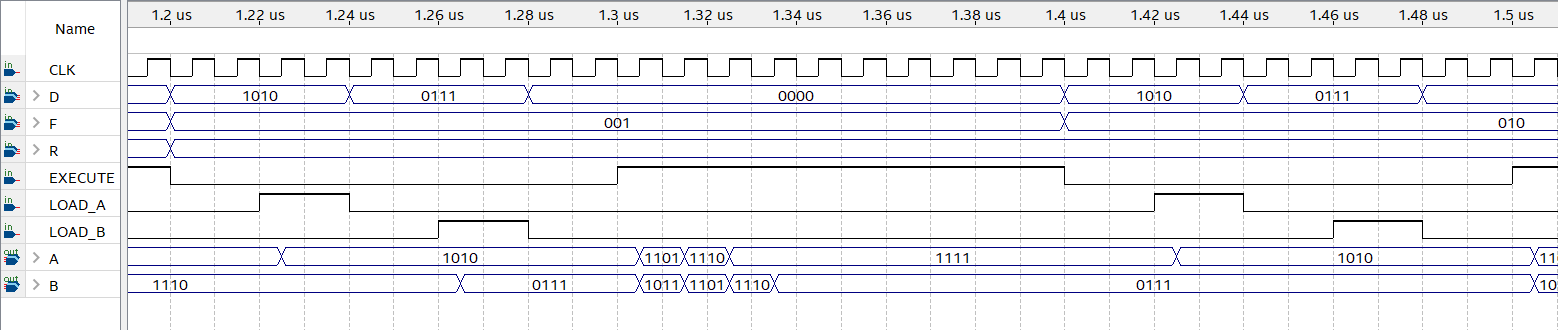
\includegraphics[width=18cm]{1200-1500.png}
    \caption{1200-1500ns}
\end{figure}
\begin{figure}[H]
    \centering
    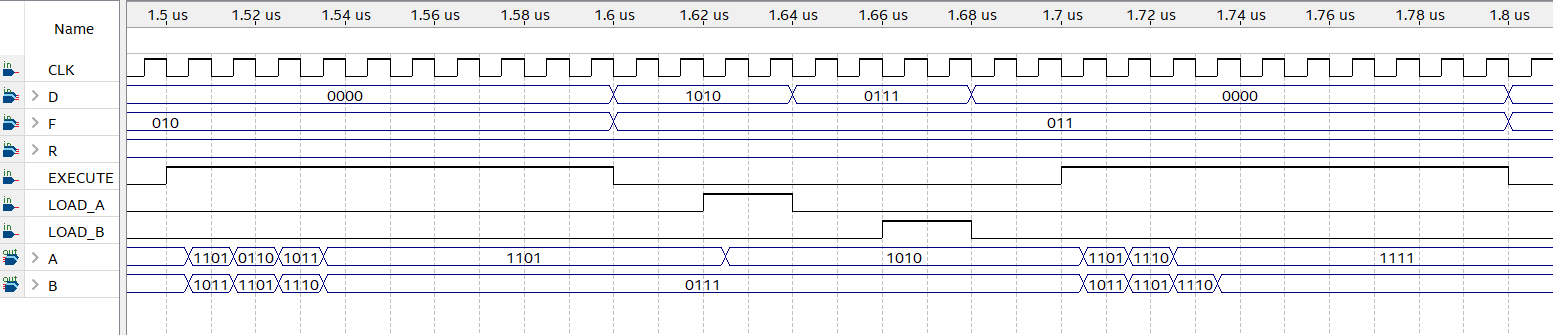
\includegraphics[width=18cm]{1500-1800.png}
    \caption{1500-1800ns}
\end{figure}
\begin{figure}[H]
    \centering
    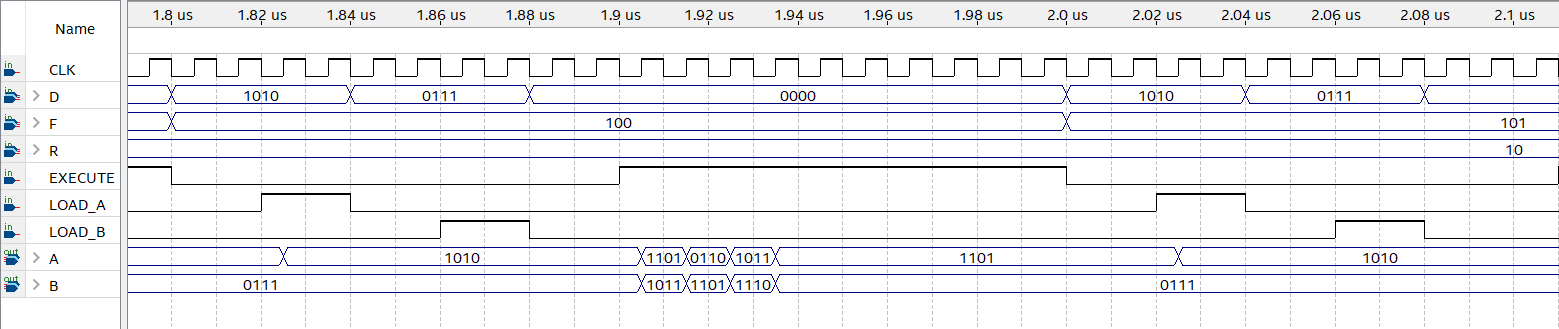
\includegraphics[width=18cm]{1800-2100.png}
    \caption{1800-2100ns}
\end{figure}
\begin{figure}[H]
    \centering
    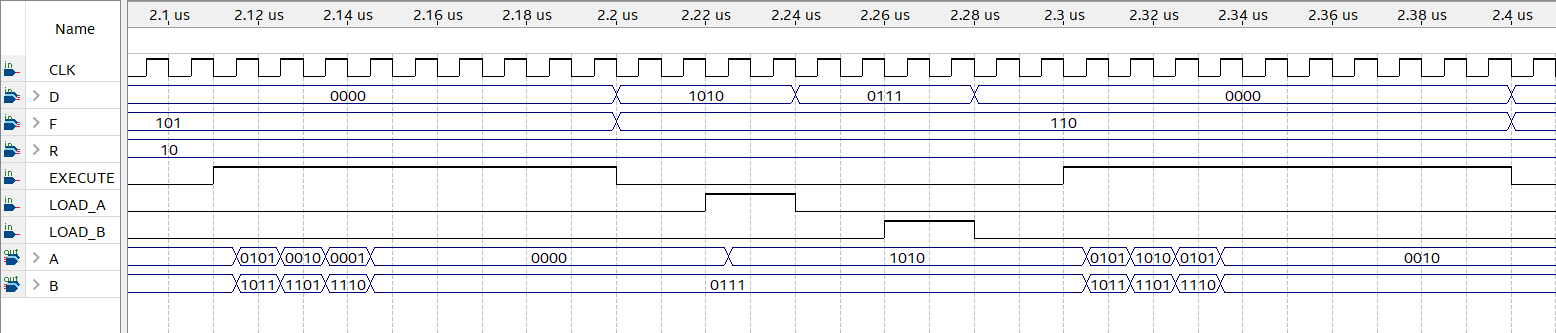
\includegraphics[width=18cm]{2100-2400.png}
    \caption{2100-2400ns}
\end{figure}
\begin{figure}[H]
    \centering
    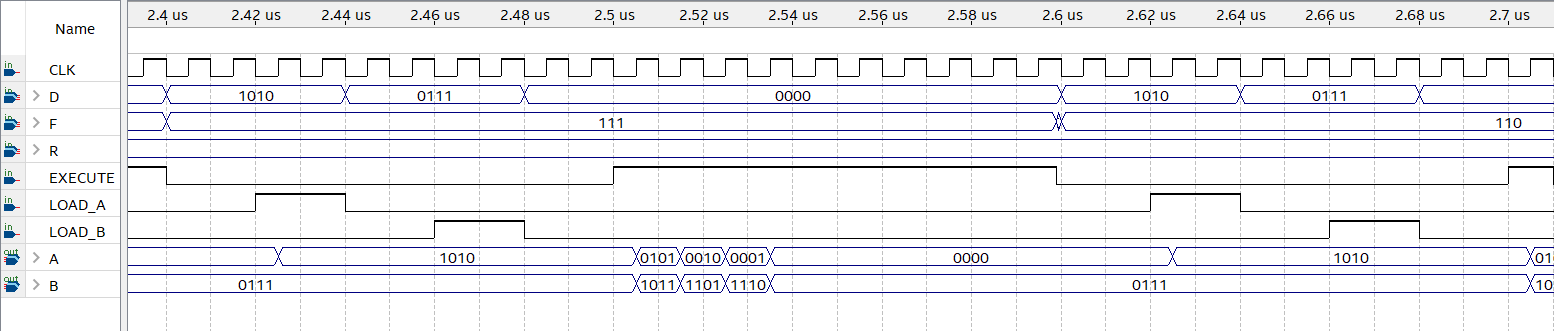
\includegraphics[width=18cm]{2400-2700.png}
    \caption{2400-2700ns}
\end{figure}
\begin{figure}[H]
    \centering
    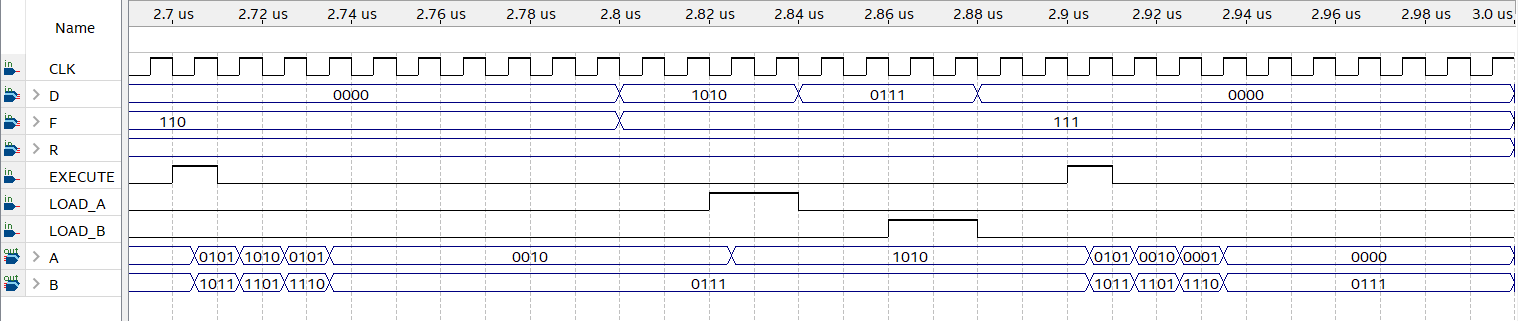
\includegraphics[width=18cm]{2700-3000.png}
    \caption{2700-3000ns}
\end{figure}

\newpage
\bibliography{lab3_ref}
\bibliographystyle{ieeetr}
\end{document}